%%%%%%%%%%%%%%%%%%%%%%%%%%%%%%%%%%%%%%%%%%%%%%%%%%%%%%%%%%%%%%%

% Set up document

\documentclass{beamer}
\usecolortheme{whale}
\setbeamersize{text margin left=5mm,text margin right=5mm}

% Used to create a section slide between section
\AtBeginSection[]{
  \begin{frame}
  \vfill
  \centering
  \begin{beamercolorbox}[sep=8pt,center,shadow=true,rounded=true]{title}
    \usebeamerfont{title}\insertsectionhead\par%
  \end{beamercolorbox}
  \vfill
  \end{frame}
}

% Remove default navigation symbols and add just  page number
\setbeamertemplate{navigation symbols}{} % Clear default navigation
\addtobeamertemplate{navigation symbols}{}{%
    \usebeamerfont{footline}%
    \usebeamercolor[fg]{footline}%
    \hspace{1em}%
    \insertframenumber/\inserttotalframenumber
}


%%%%%%%%%%%%%%%%%%%%%%%%%%%%%%%%%%%%%%%%%%%%%%%%%%%%%%%%%%%%%%%

% Title page

\title{Stroke Audit Machine Learning (SAMueL) \\ Workshop 1}
\subtitle{Investigating variation in clinical decision-making with explainable AI}


\author{Kerry Pearn\inst{1}, Michael Allen\inst{1}, Anna Laws\inst{1}, Keira Pratt-Boyden\inst{1}, Martin James\inst{1,2} }
\institute{\inst{1} University of Exeter Medical School \inst{2} Royal Devon University Healthcare NHS Foundation Trust}

%\institute{Overleaf}
\date{November 2022}


\begin{document}

%\frame{\titlepage}

\begin{frame}
\titlepage


\end{frame}

%%%%%%%%%%%%%%%%%%%%%%%%%%%%%%%%%%%%%%%%%%%%%%%%%%%%%%%%%%%%%%%

\begin{frame}{What will we cover?}


\begin{itemize}
    \setlength\itemsep{1mm}
    \item What's the problem?
    \item What's the question?
    \item Modelling the emergency stroke pathway
    \item Machine learning overview
    \item Model accuracy and simplification
    \item SHAP?
    \item Drivers of thrombolysis across all hospitals
    \item Example patients - what do different hospitals do? What would you do?
    \item General discussion (but please feel very free to ask questions, or comments, as we go along!)
\end{itemize}

\end{frame}

%%%%%%%%%%%%%%%%%%%%%%%%%%%%%%%%%%%%%%%%%%%%%%%%%%%%%%%%%%%%%%%

\begin{frame}{What's the problem?}


\begin{itemize}
    \setlength\itemsep{5mm}
    \item Thrombolysis rates in England and Wales are stable at 11-12\% against a NHS Long Term Plan target of 20\%.
    \item Thrombolysis rates at individual hospitals range from 5\% to 25\%.
\end{itemize}


\end{frame}

%%%%%%%%%%%%%%%%%%%%%%%%%%%%%%%%%%%%%%%%%%%%%%%%%%%%%%%%%%%%%%%

\begin{frame}{What's the question?}

What causes this variation in thrombolysis rates, and what could reasonably be achieved at each hospital (allowing for each hospital's own patient population)?


\vspace{10mm}
\begin{quote}
  ``Your decision to treat or not treat … That’s the difficult part.\\
  That’s the grey area where everyone does a different thing.''\\
  \hfill\footnotesize\textnormal{— Stroke Consultant during interviews for SAMueL}
\end{quote}


\end{frame}

%%%%%%%%%%%%%%%%%%%%%%%%%%%%%%%%%%%%%%%%%%%%%%%%%%%%%%%%%%%%%%%

\begin{frame}
\frametitle{Breaking down the emergency stroke pathway into key steps}
\begin{center}
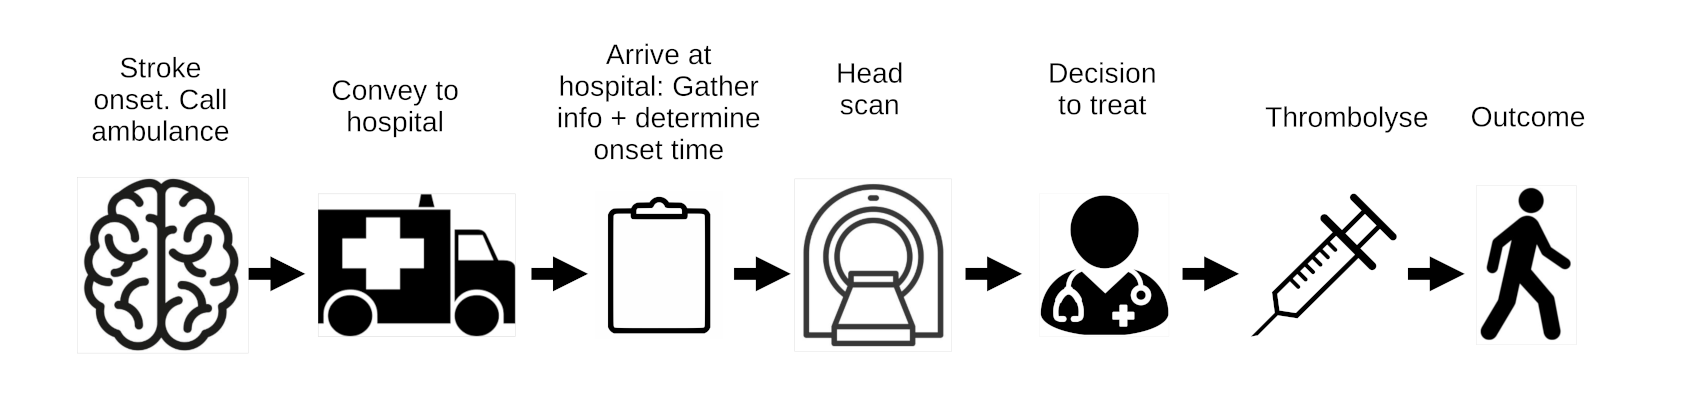
\includegraphics[width=1.0\textwidth]{./images/pathway}
\end{center}
We can model key changes to pathway:
\begin{small}
\begin{itemize}
    \item What if the pathway were faster?
    \item What if hospital determined the stroke onset time in more patients?
    \item What if clinical decision-making was like that of \emph{benchmark} hospitals? (Predict what treatment a patient would receive at other hospitals).
\end{itemize}
\end{small}
\footnotesize{We model these changes with a hospital's own patient population, to allow for inter-hospital variation in patient population characteristics.}
\end{frame}

%%%%%%%%%%%%%%%%%%%%%%%%%%%%%%%%%%%%%%%%%%%%%%%%%%%%%%%%%%%%%%%

\begin{frame}
\frametitle{Machine learning overview}
\begin{center}
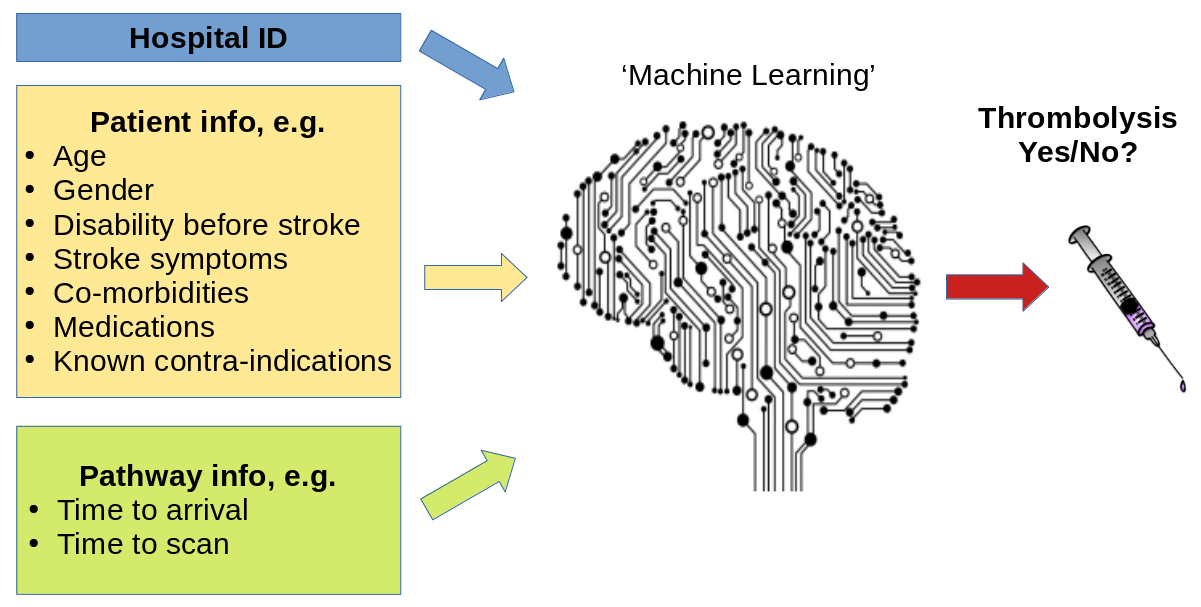
\includegraphics[width=0.90\textwidth]{./images/ml_model_high_level}
\end{center}


Machine learning (and nearly all \emph{artificial intelligence}) is based on the simple principle of recognising similarity to what has been seen before.
\vspace{3mm}

We accessed 240,000 emergency stroke admissions in England and Wales over three years.
\end{frame}

%%%%%%%%%%%%%%%%%%%%%%%%%%%%%%%%%%%%%%%%%%%%%%%%%%%%%%%%%%%%%%%

\begin{frame}{Model accuracy, and simplification}

Our machine learning models use XGBoost classification, and are based on all patients who arrive within 4 hours of known stroke onset.

\vspace{5mm}

\begin{columns}[T] % [T] Top aligns columns

    \begin{column}{0.5\textwidth}
    
        The full model has 61 patient features:
        
        \begin{footnotesize}
        \begin{itemize}
            \item Overall accuracy = 85.2\%
            \item Best combined sensitivity and specificity = 84.3\%
            \item ROC AUC = 0.921
        \end{itemize}
        \end{footnotesize}
        
        \vspace{3mm}
        
        A simplified model with 8 features
        
        \begin{footnotesize}
        \begin{itemize}
            \item Overall accuracy = 84.8\%
            \item Best combined sensitivity and specificity = 83.8\%
            \item ROC AUC = 0.916
        \end{itemize}
        \end{footnotesize}
    \end{column}
    
    \begin{column}{0.5\textwidth}
    The 8 features of the simplified model are:
        \begin{footnotesize}
        \begin{enumerate}
            \item Arrival-to-scan time
            \item Stroke type (infarction/haemorrhage)
            \item Stroke severity (NIHSS)
            \item Precise or estimated stroke onset time
            \item Prior disability level (mRS)
            \item Stroke team
            \item Use of AF anticoagulants
            \item Onset-to-arrival time
        \end{enumerate}
        \end{footnotesize}
        
    \vspace{2mm}
    \tiny{There are only very weak correlations between the selected features with no R-squared being greater than 0.05.}
    \end{column}
    
\end{columns}
\end{frame}


%%%%%%%%%%%%%%%%%%%%%%%%%%%%%%%%%%%%%%%%%%%%%%%%%%%%%%%%%%%%%%%

\begin{frame}
\frametitle{Explaining model predictions with SHAP values}

SHAP values show the influence of features (even for \emph{`black box'} models).

\begin{center}
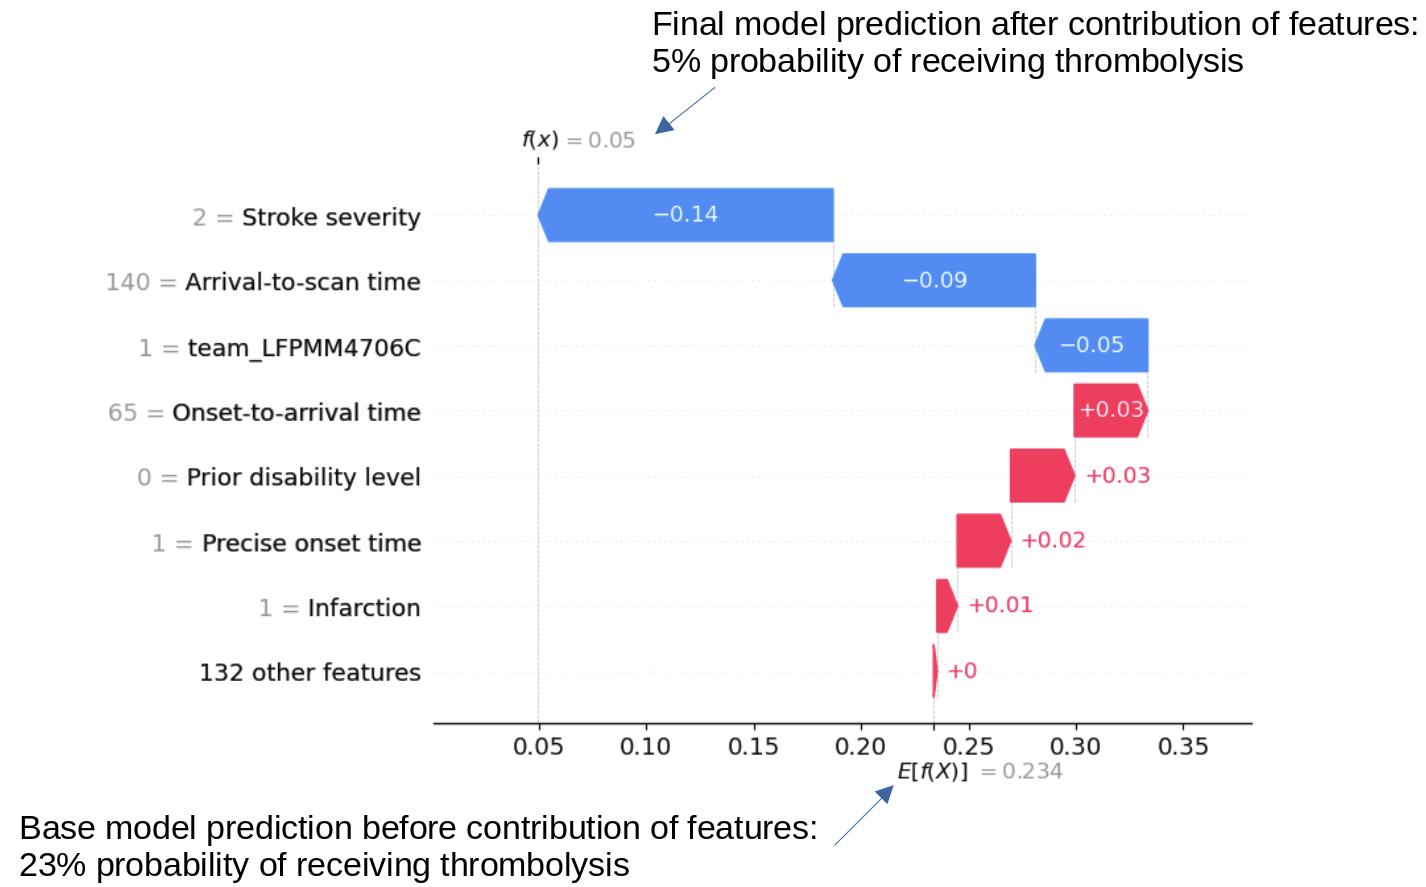
\includegraphics[width=0.85\textwidth]{./images/xgb_waterfall_low_probability.jpg}
\end{center}
\end{frame}


%%%%%%%%%%%%%%%%%%%%%%%%%%%%%%%%%%%%%%%%%%%%%%%%%%%%%%%%%%%%%%%

\begin{frame}
\frametitle{What drives use of thrombolysis across all hospitals?}

\footnotesize{Note: SHAP values here are \emph{log odds}. Each step-change in value of \textpm 1 changes the chances of receiving thrombolysis about 3-fold. (Plots are in order of feature importance.)}

\begin{center}
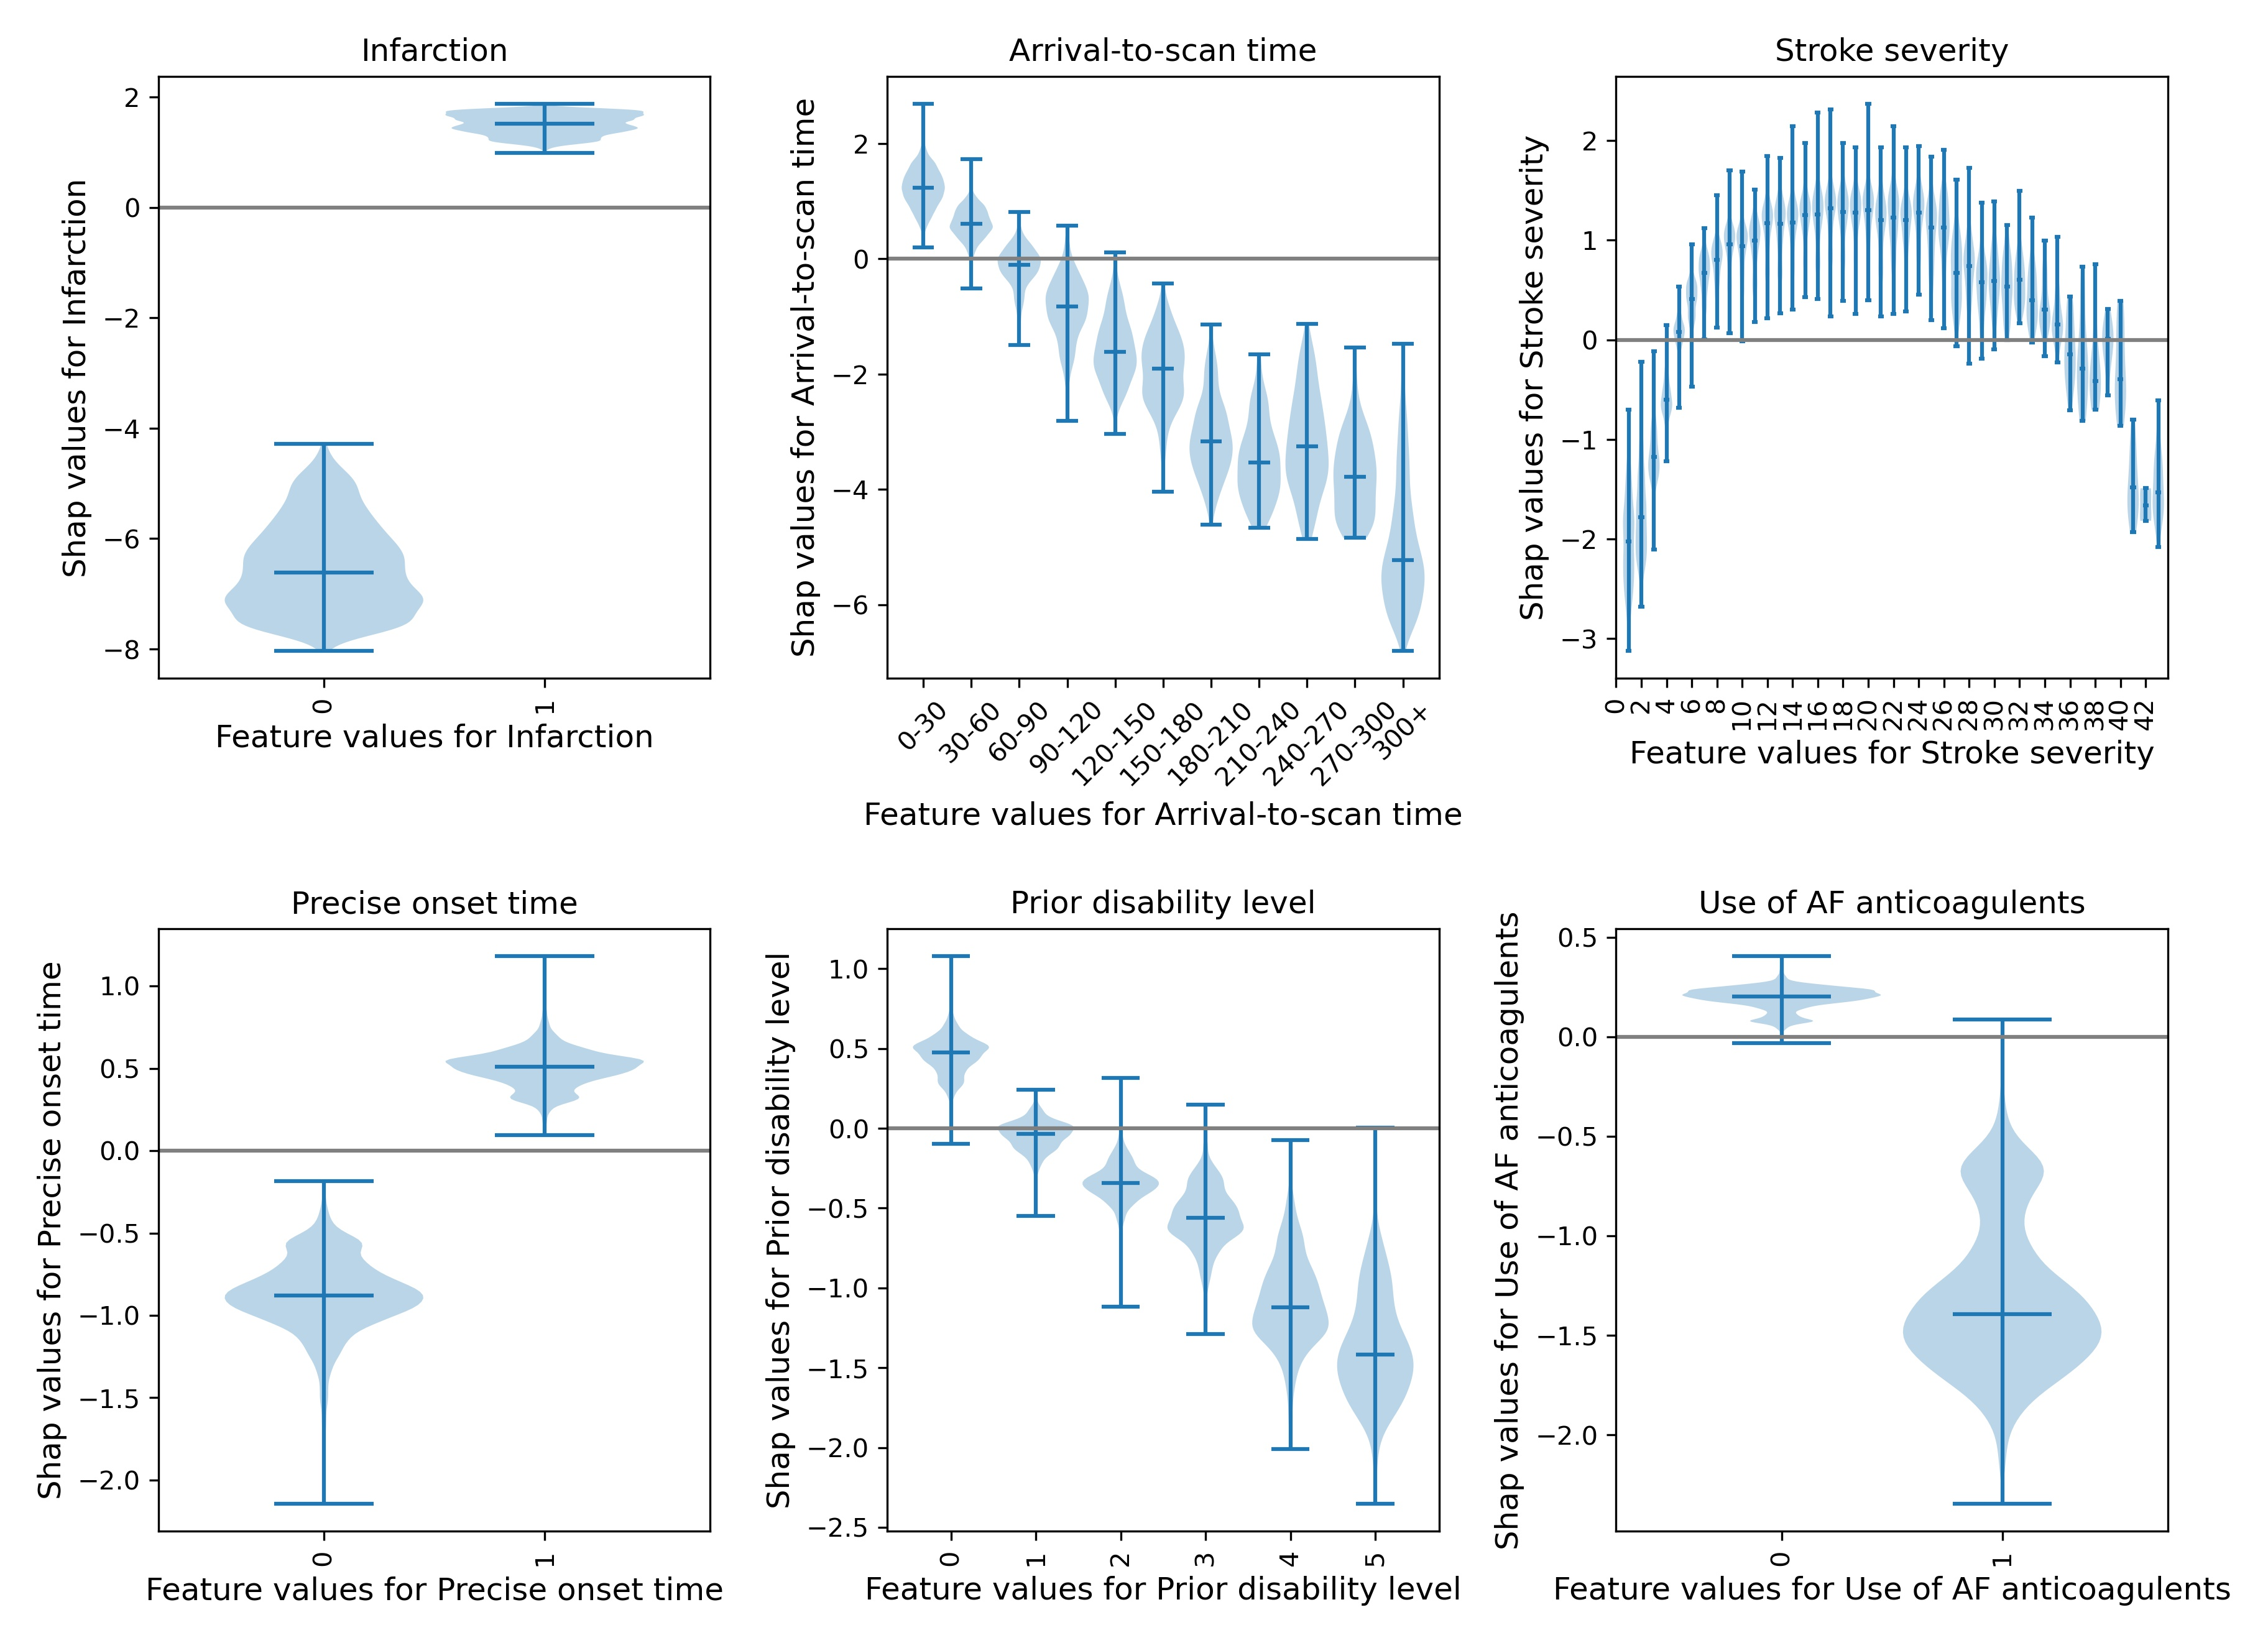
\includegraphics[width=0.80\textwidth]{./images/xgb_thrombolysis_shap_violin.jpg}
\end{center}
\end{frame}

%%%%%%%%%%%%%%%%%%%%%%%%%%%%%%%%%%%%%%%%%%%%%%%%%%%%%%%%%%%%%%%

\begin{frame}
\frametitle{Investigating how hospitals differ in thrombolysis decision-making (Patient 1: Base patient)}

Assuming there are no reasons not stated here to exclude a patient from use of thrombolysis, would you give this patient thrombolysis?

\vspace{3mm}

\begin{columns}
    \begin{column}{0.6\textwidth}
        \begin{itemize}
            \item Onset to arrival = 80 mins
            \item Arrival to scan = 20 mins
            \item Infarction = Yes
            \item NIHSS = 15
            \item Prior disability level = 0
            \item Precise onset time = Yes
            \item Use of AF anticoagulents = No
        \end{itemize}
    \end{column}
    
    \begin{column}{0.4\textwidth}
    
    \end{column}

\end{columns}
\end{frame}


\begin{frame}
\frametitle{Investigating how hospitals differ in thrombolysis decision-making (Patient 1: Base patient)}

Assuming there are no reasons not stated here to exclude a patient from use of thrombolysis, would you give this patient thrombolysis?
\vspace{3mm}

\begin{columns}
    \begin{column}{0.5\textwidth}
        \begin{itemize}
            \item Onset to arrival = 80 mins
            \item Arrival to scan = 20 mins
            \item Infarction = Yes
            \item NIHSS = 15
            \item Prior disability level = 0
            \item Precise onset time = Yes
            \item Use of AF anticoagulents = No
        \end{itemize}
    \end{column}
    
    \begin{column}{0.4\textwidth}
    Our model predicts 131 out of 132 (99\%) hospitals would give this patient thrombolysis.
    \end{column}

\end{columns}
\end{frame}

%%%%%%%%%%%%%%%%%%%%%%%%%%%%%%%%%%%%%%%%%%%%%%%%%%%%%%%%%%%%%%%

\begin{frame}
\frametitle{Investigating how hospitals differ in thrombolysis decision-making (Patient 2: Milder stroke)}

Assuming there are no reasons not stated here to exclude a patient from use of thrombolysis, would you give this patient thrombolysis?

\vspace{3mm}

\begin{columns}
    \begin{column}{0.6\textwidth}
        \begin{itemize}
            \item Onset to arrival = 80 mins
            \item Arrival to scan = 20 mins
            \item Infarction = Yes
            \item \emph{NIHSS = 4}
            \item Prior disability level = 0
            \item Precise onset time = Yes
            \item Use of AF anticoagulents = No
        \end{itemize}
    \end{column}
    
    \begin{column}{0.4\textwidth}
    
    \end{column}

\end{columns}
\end{frame}


\begin{frame}
\frametitle{Investigating how hospitals differ in thrombolysis decision-making (Patient 2: Milder stroke)}

Assuming there are no reasons not stated here to exclude a patient from use of thrombolysis, would you give this patient thrombolysis?

\vspace{3mm}

\begin{columns}
    \begin{column}{0.5\textwidth}
        \begin{itemize}
            \item Onset to arrival = 80 mins
            \item Arrival to scan = 20 mins
            \item Infarction = Yes
            \item \emph{NIHSS = 4}
            \item Prior disability level = 0
            \item Precise onset time = Yes
            \item Use of AF anticoagulents = No
        \end{itemize}
    \end{column}
    
    \begin{column}{0.4\textwidth}
    Our model predicts 97 out of 132 (73\%) hospitals would give this patient thrombolysis.
    \end{column}

\end{columns}
\end{frame}

%%%%%%%%%%%%%%%%%%%%%%%%%%%%%%%%%%%%%%%%%%%%%%%%%%%%%%%%%%%%%%%

\begin{frame}
\frametitle{Investigating how hospitals differ in thrombolysis decision-making (Patient 3: Pre-stroke disability)}

Assuming there are no reasons not stated here to exclude a patient from use of thrombolysis, would you give this patient thrombolysis?

\vspace{3mm}


\begin{columns}
    \begin{column}{0.5\textwidth}
        \begin{itemize}
            \item Onset to arrival = 80 mins
            \item Arrival to scan = 20 mins
            \item Infarction = Yes
            \item NIHSS = 15
            \item \emph{Prior disability level = 3*}
            \item Precise onset time = Yes
            \item Use of AF anticoagulents = No
        \end{itemize}
    \vspace{3mm}    
    \footnotesize{*Moderate disability; requires some help, but able to walk without assistance.}
    \end{column}
    
    \begin{column}{0.4\textwidth}
    
    \end{column}

\end{columns}
\end{frame}

%%%%%%%%%%%%%%%%%%%%%%%%%%%%%%%%%%%%%%%%%%%%%%%%%%%%%%%%%%%%%%%

\begin{frame}
\frametitle{Investigating how hospitals differ in thrombolysis decision-making (Patient 3: Pre-stroke disability)}

Assuming there are no reasons not stated here to exclude a patient from use of thrombolysis, would you give this patient thrombolysis?

\vspace{3mm}

\begin{columns}
    \begin{column}{0.5\textwidth}
        \begin{itemize}
            \item Onset to arrival = 80 mins
            \item Arrival to scan = 20 mins
            \item Infarction = Yes
            \item NIHSS = 15
            \item \emph{Prior disability level = 3*}
            \item Precise onset time = Yes
            \item Use of AF anticoagulents = No
        \end{itemize}
    \vspace{3mm}    
    \footnotesize{*Moderate disability; requires some help, but able to walk without assistance.}
    \end{column}
    
    \begin{column}{0.4\textwidth}
    Our model predicts 114 out of 132 (86\%) hospitals would give this patient thrombolysis.
    \end{column}

\end{columns}
\end{frame}

%%%%%%%%%%%%%%%%%%%%%%%%%%%%%%%%%%%%%%%%%%%%%%%%%%%%%%%%%%%%%%%

\begin{frame}
\frametitle{Investigating how hospitals differ in thrombolysis decision-making (Patient 4: Estimated stroke onset time)}

Assuming there are no reasons not stated here to exclude a patient from use of thrombolysis, would you give this patient thrombolysis?

\vspace{3mm}

\begin{columns}
    \begin{column}{0.6\textwidth}
        \begin{itemize}
            \item Onset to arrival = 80 mins
            \item Arrival to scan = 20 mins
            \item Infarction = Yes
            \item NIHSS = 15
            \item Prior disability level = 0
            \item \emph{Precise onset time = No}
            \item Use of AF anticoagulents = No
        \end{itemize}
    \end{column}
    
    \begin{column}{0.4\textwidth}
    
    \end{column}

\end{columns}
\end{frame}


\begin{frame}
\frametitle{Investigating how hospitals differ in thrombolysis decision-making (Patient 4: Estimated stroke onset time)}

Assuming there are no reasons not stated here to exclude a patient from use of thrombolysis, would you give this patient thrombolysis?

\vspace{3mm}

\begin{columns}
    \begin{column}{0.5\textwidth}
        \begin{itemize}
            \item Onset to arrival = 80 mins
            \item Arrival to scan = 20 mins
            \item Infarction = Yes
            \item NIHSS = 15
            \item Prior disability level = 0
            \item \emph{Precise onset time = No}
            \item Use of AF anticoagulents = No
        \end{itemize}
    \end{column}
    
    \begin{column}{0.4\textwidth}
    Our model predicts 84 out of 132 (64\%) hospitals would give this patient thrombolysis.
    \end{column}

\end{columns}
\end{frame}


%%%%%%%%%%%%%%%%%%%%%%%%%%%%%%%%%%%%%%%%%%%%%%%%%%%%%%%%%%%%%%%
\begin{frame}
\frametitle{Key findings}
General observations about thrombolysis use: The chance of receiving thrombolysis is increased by:
\emph{
\begin{itemize}
    \item Shorter arrival-to-scan times
    \item Mid-level stroke severity
    \item Precise onset time
    \item Lower pre-stroke disability
\end{itemize}
}

\vspace{5mm}

Lower thrombolysing units are particularly less likely to give thrombolysis to patients with:
\emph{
\begin{itemize}
    \item Low or high stroke severity
    \item Higher pre-stroke disability
    \item Estimated onset time
\end{itemize}
}

\end{frame}

%%%%%%%%%%%%%%%%%%%%%%%%%%%%%%%%%%%%%%%%%%%%%%%%%%%%%%%%%%%%%%%
\begin{frame}
\frametitle{Possible questions for discussion - but please comment as you wish!}
\begin{small}
\begin{itemize}
\setlength\itemsep{1mm}
    \item Does anything surprise you here, and do these findings reflect your own experiences?
    \item What are your experiences in treating mild strokes and patients with estimated stroke-onset times?
    \item What might you do with the knowledge that different hospitals have different attitudes to mild strokes and patients with estimated stroke-onset times? Would it stimulate you to consider your own practice?
    \item Why do you think pre-stroke disability appears influential in thrombolysis decision-making?
    \item Do you find SHAP understandable?
    \item Do the patient examples help? Would you like them filled out more, or do you prefer to see the key decision-makign data in the model?
\end{itemize}
\end{small}
\end{frame}

%%%%%%%%%%%%%%%%%%%%%%%%%%%%%%%%%%%%%%%%%%%%%%%%%%%%%%%%%%%%%%%
\begin{frame}{Thank you!!}
    Thank you for your time and attention!
\end{frame}

%%%%%%%%%%%%%%%%%%%%%%%%%%%%%%%%%%%%%%%%%%%%%%%%%%%%%%%%%%%%%%%


% EXTRA SLIDE(S)

\begin{frame}{Reserve slides}
    
\end{frame}

%%%%%%%%%%%%%%%%%%%%%%%%%%%%%%%%%%%%%%%%%%%%%%%%%%%%%%%%%%%%%%%%%

\begin{frame}
\frametitle{When will low thrombolysing units not use thrombolysis when higher thrombolysing would?}

\footnotesize{Here, a high SHAP shows when a low-thrombolysing unit will reject use of thrombolysis when a higher thrombolysing hospital would use thrombolysis. (Plots are in order of feature importance.)}

\begin{center}
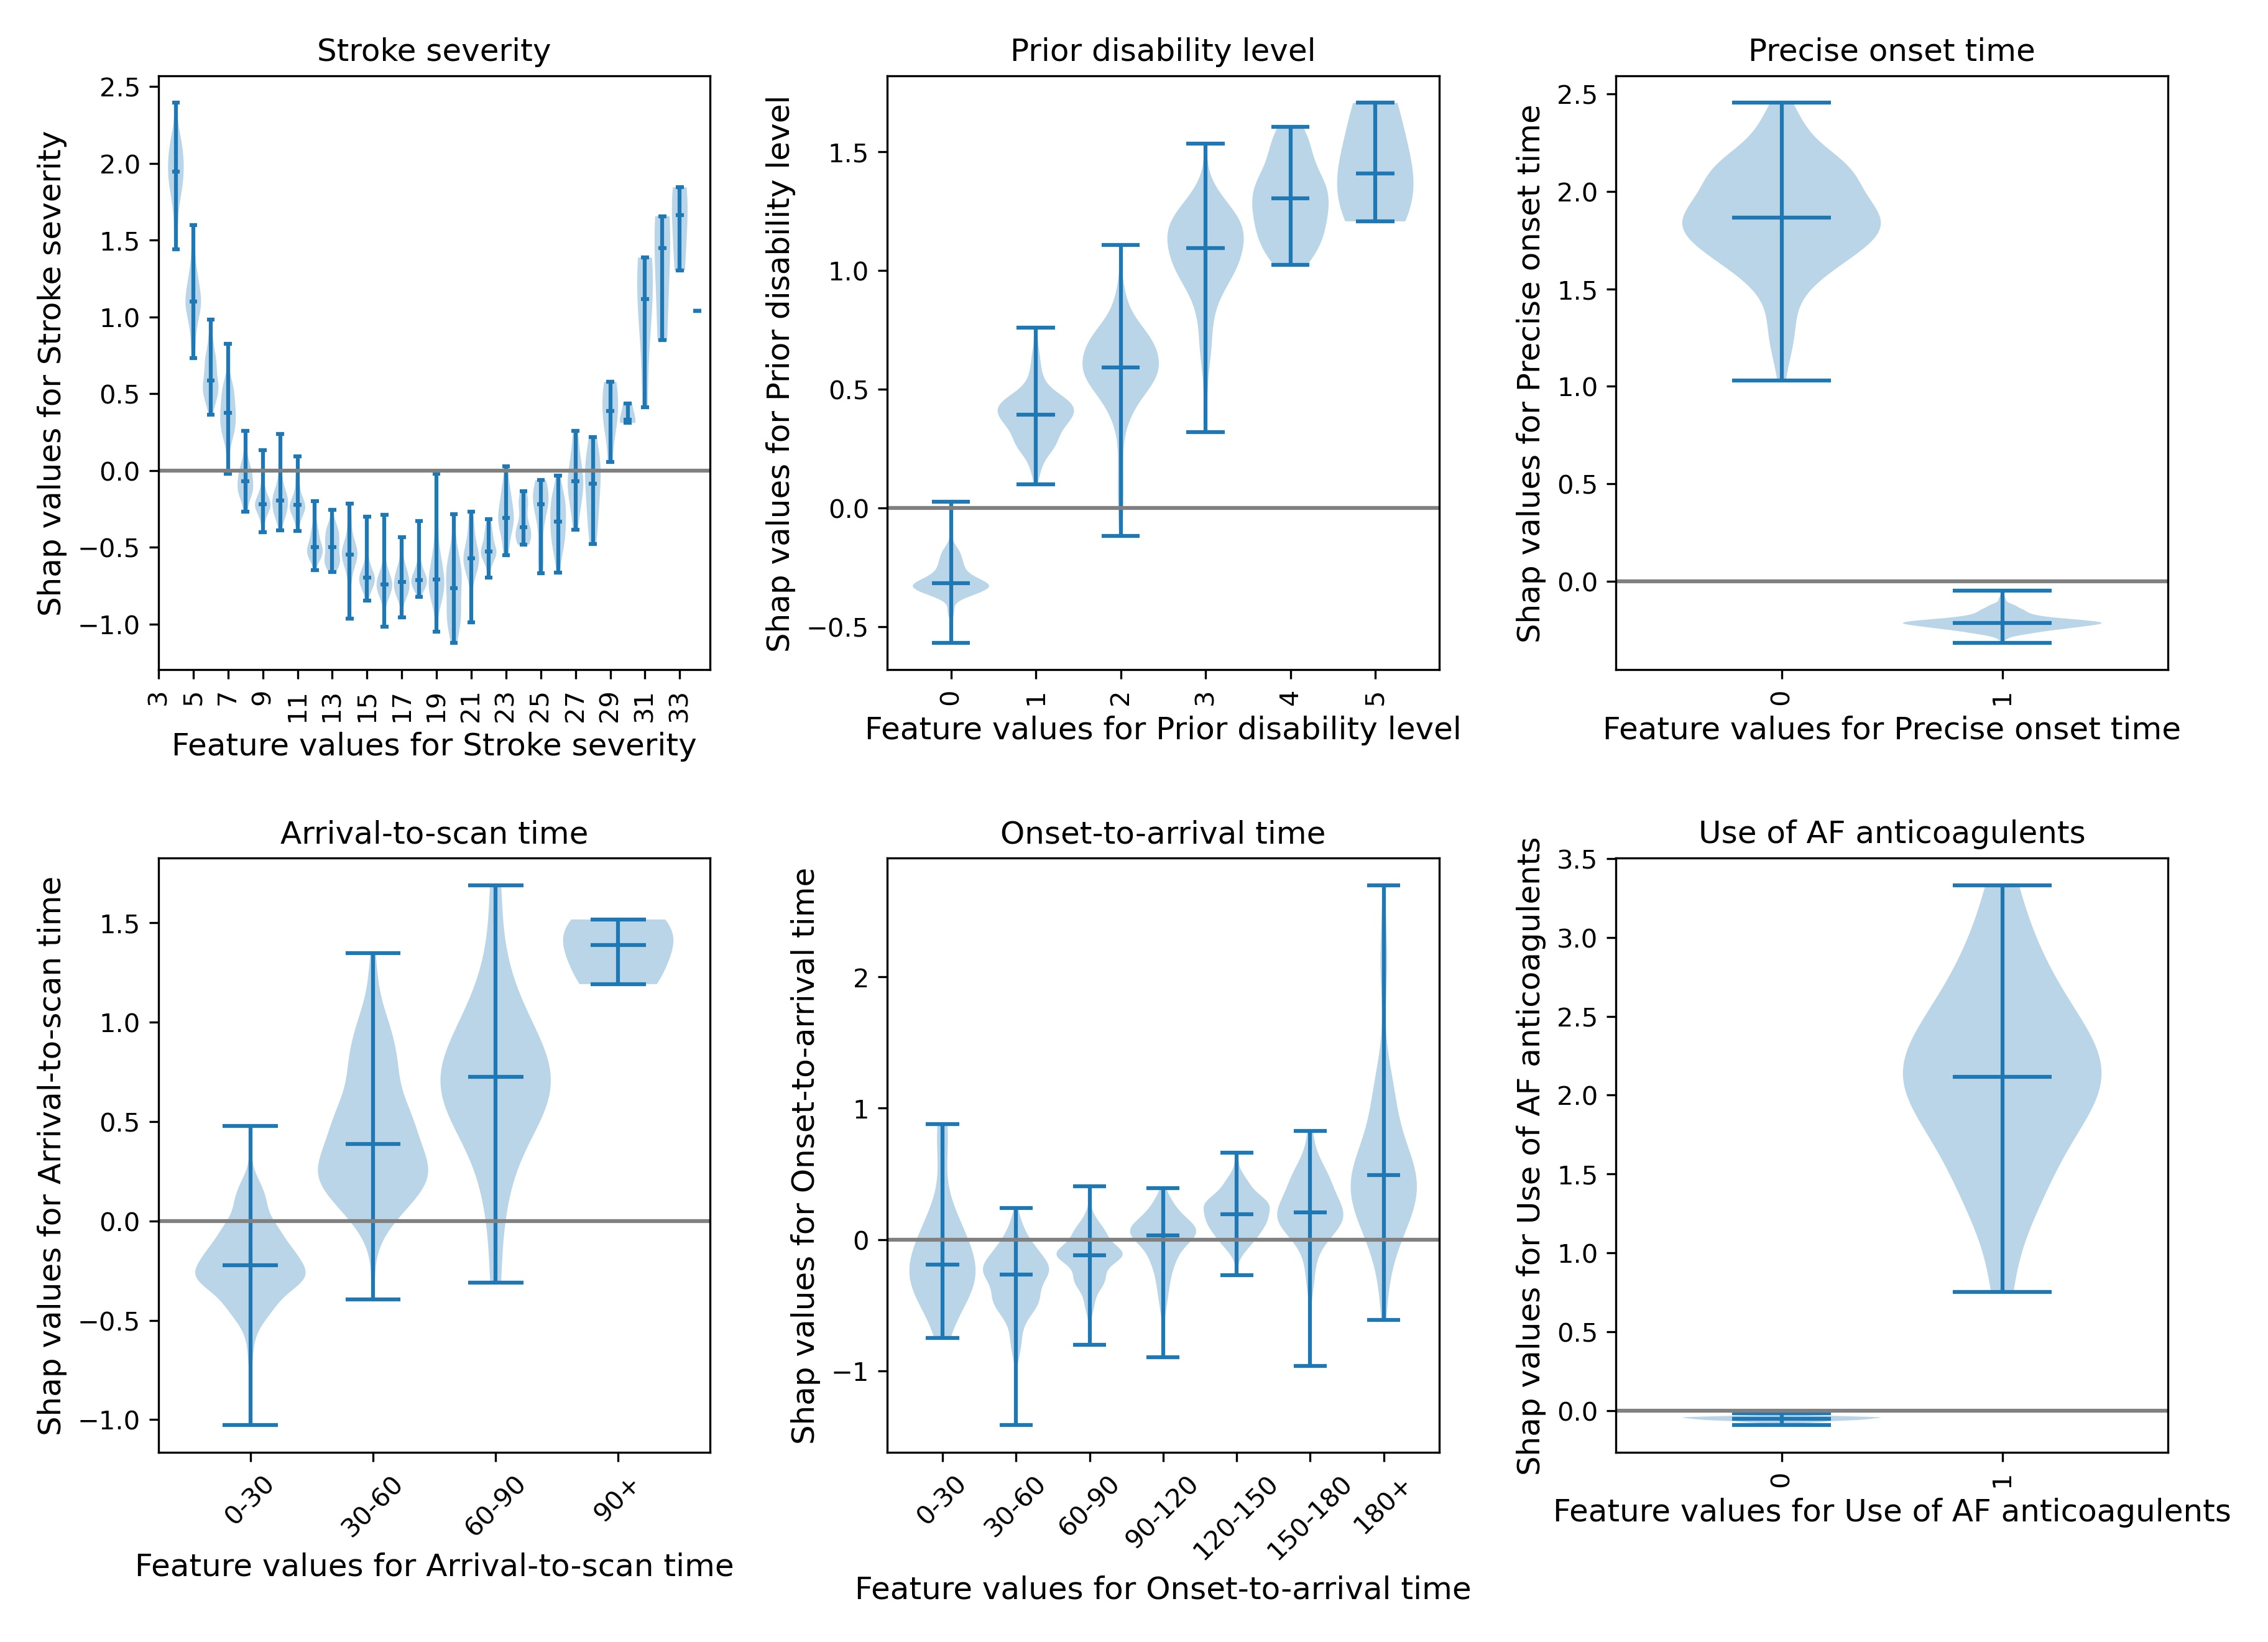
\includegraphics[width=0.75\textwidth]{./images/xgb_predicting_difference_shap_violin.jpg}
\end{center}
\end{frame}



\end{document}




